\part{Using SIFT for Image Matching}\label{part:Matching descriptors}

基于前面提取\sift 特征点、描述\sift 特征点的过程,本部分进一步介绍如何进行多视角图像间特征点的匹配,并展示一个最终的实验结果。

\section{描述子匹配}

寻找一幅图像中某个特征点在另一幅图像中的对应,即寻找与之描述子最为接近的特征点。衡量两个描述子(即特征向量)之间距离的方式有很多,例如欧氏距离(2-范数),汉明距离等。这里,可直接使用欧氏距离,并且以暴力匹配的方式寻找描述子之间的匹配关系。

同时,不一定一幅图像中的每一个描述子都能在另一幅图像中找到对应点,因此可以对描述子之间的距离设置一个上限;并且可以每次选取距离最近的两个描述子,如果最接近的描述子距离上要明显小于次接近的描述子,则可认为最接近的描述子是可靠的。

\section{实验:图像SIFT特征匹配}

该部分大致介绍代码框架及代码实现,并通过从命令行执行脚本的方式,对\sift 特征点提取、图像\sift 特征点匹配算法进行了实验验证。实验平台\texttt{NVIDIA® Jetson AGX Orin™ Developer Kit},\texttt{CUDA 11.4},实验图像分辨率$760\times 570$。

\subsection{代码库介绍}

目前使用\texttt{Python}实现了前面介绍的关于\sift 特征提取、描述与匹配等基本方法。代码参考自苏黎世大学\zhparen{UZH}\emph{2022年秋季移动机器人视觉算法}课程\footnote{课程网站:https://rpg.ifi.uzh.ch/teaching.html},在其提供代码的基础上,对构造高斯金字塔、生成特征描述子等过程均进行了优化。算法被封装在\texttt{sift}目录下,形成一个\texttt{Python}包,可以在其他脚本文件中通过\texttt{import}调用其所实现的\sift 特征提取和匹配方法。

\texttt{sift}目录下各文件介绍:
\begin{zshcode}
.
├── __init__.py  # 包(package)标识文件
├── descriptor.py  # 计算特征描述子
├── mysift.py  # 匹配描述子
└── pyramid.py  # 构建DoG Pyramid,并提取SIFT特征点
\end{zshcode}

环境安装说明:
\begin{zshcode}
# 创建conda虚拟环境
conda create -n mysift python=3.8 numpy
# 进入conda虚拟环境
conda activate mysift
# 安装opencv
pip install opencv-python
\end{zshcode}

\subsection{提取特征点}

输入一幅图像,提取其中的\sift 关键点。脚本运行命令示例:
\begin{zshcode}
python sift_detect.py \
       --file_dir images/nvidia-3.jpg \ # input image
       -o 5 \ # number of octaves
       -s 3 \ # number of scales per octave
       -rescale 0.3 \ # rescale images to make it faster
       --sigma 1.0 \ # use for Gaussian blurring
       --output_dir images/experiment/nvidia-3-keypoints.jpg \ # output destination
       -t 5e-2 # threshold for detection
\end{zshcode}

\begin{figure}[H]
    \centering
    \subfigure[输入的原图像]{
        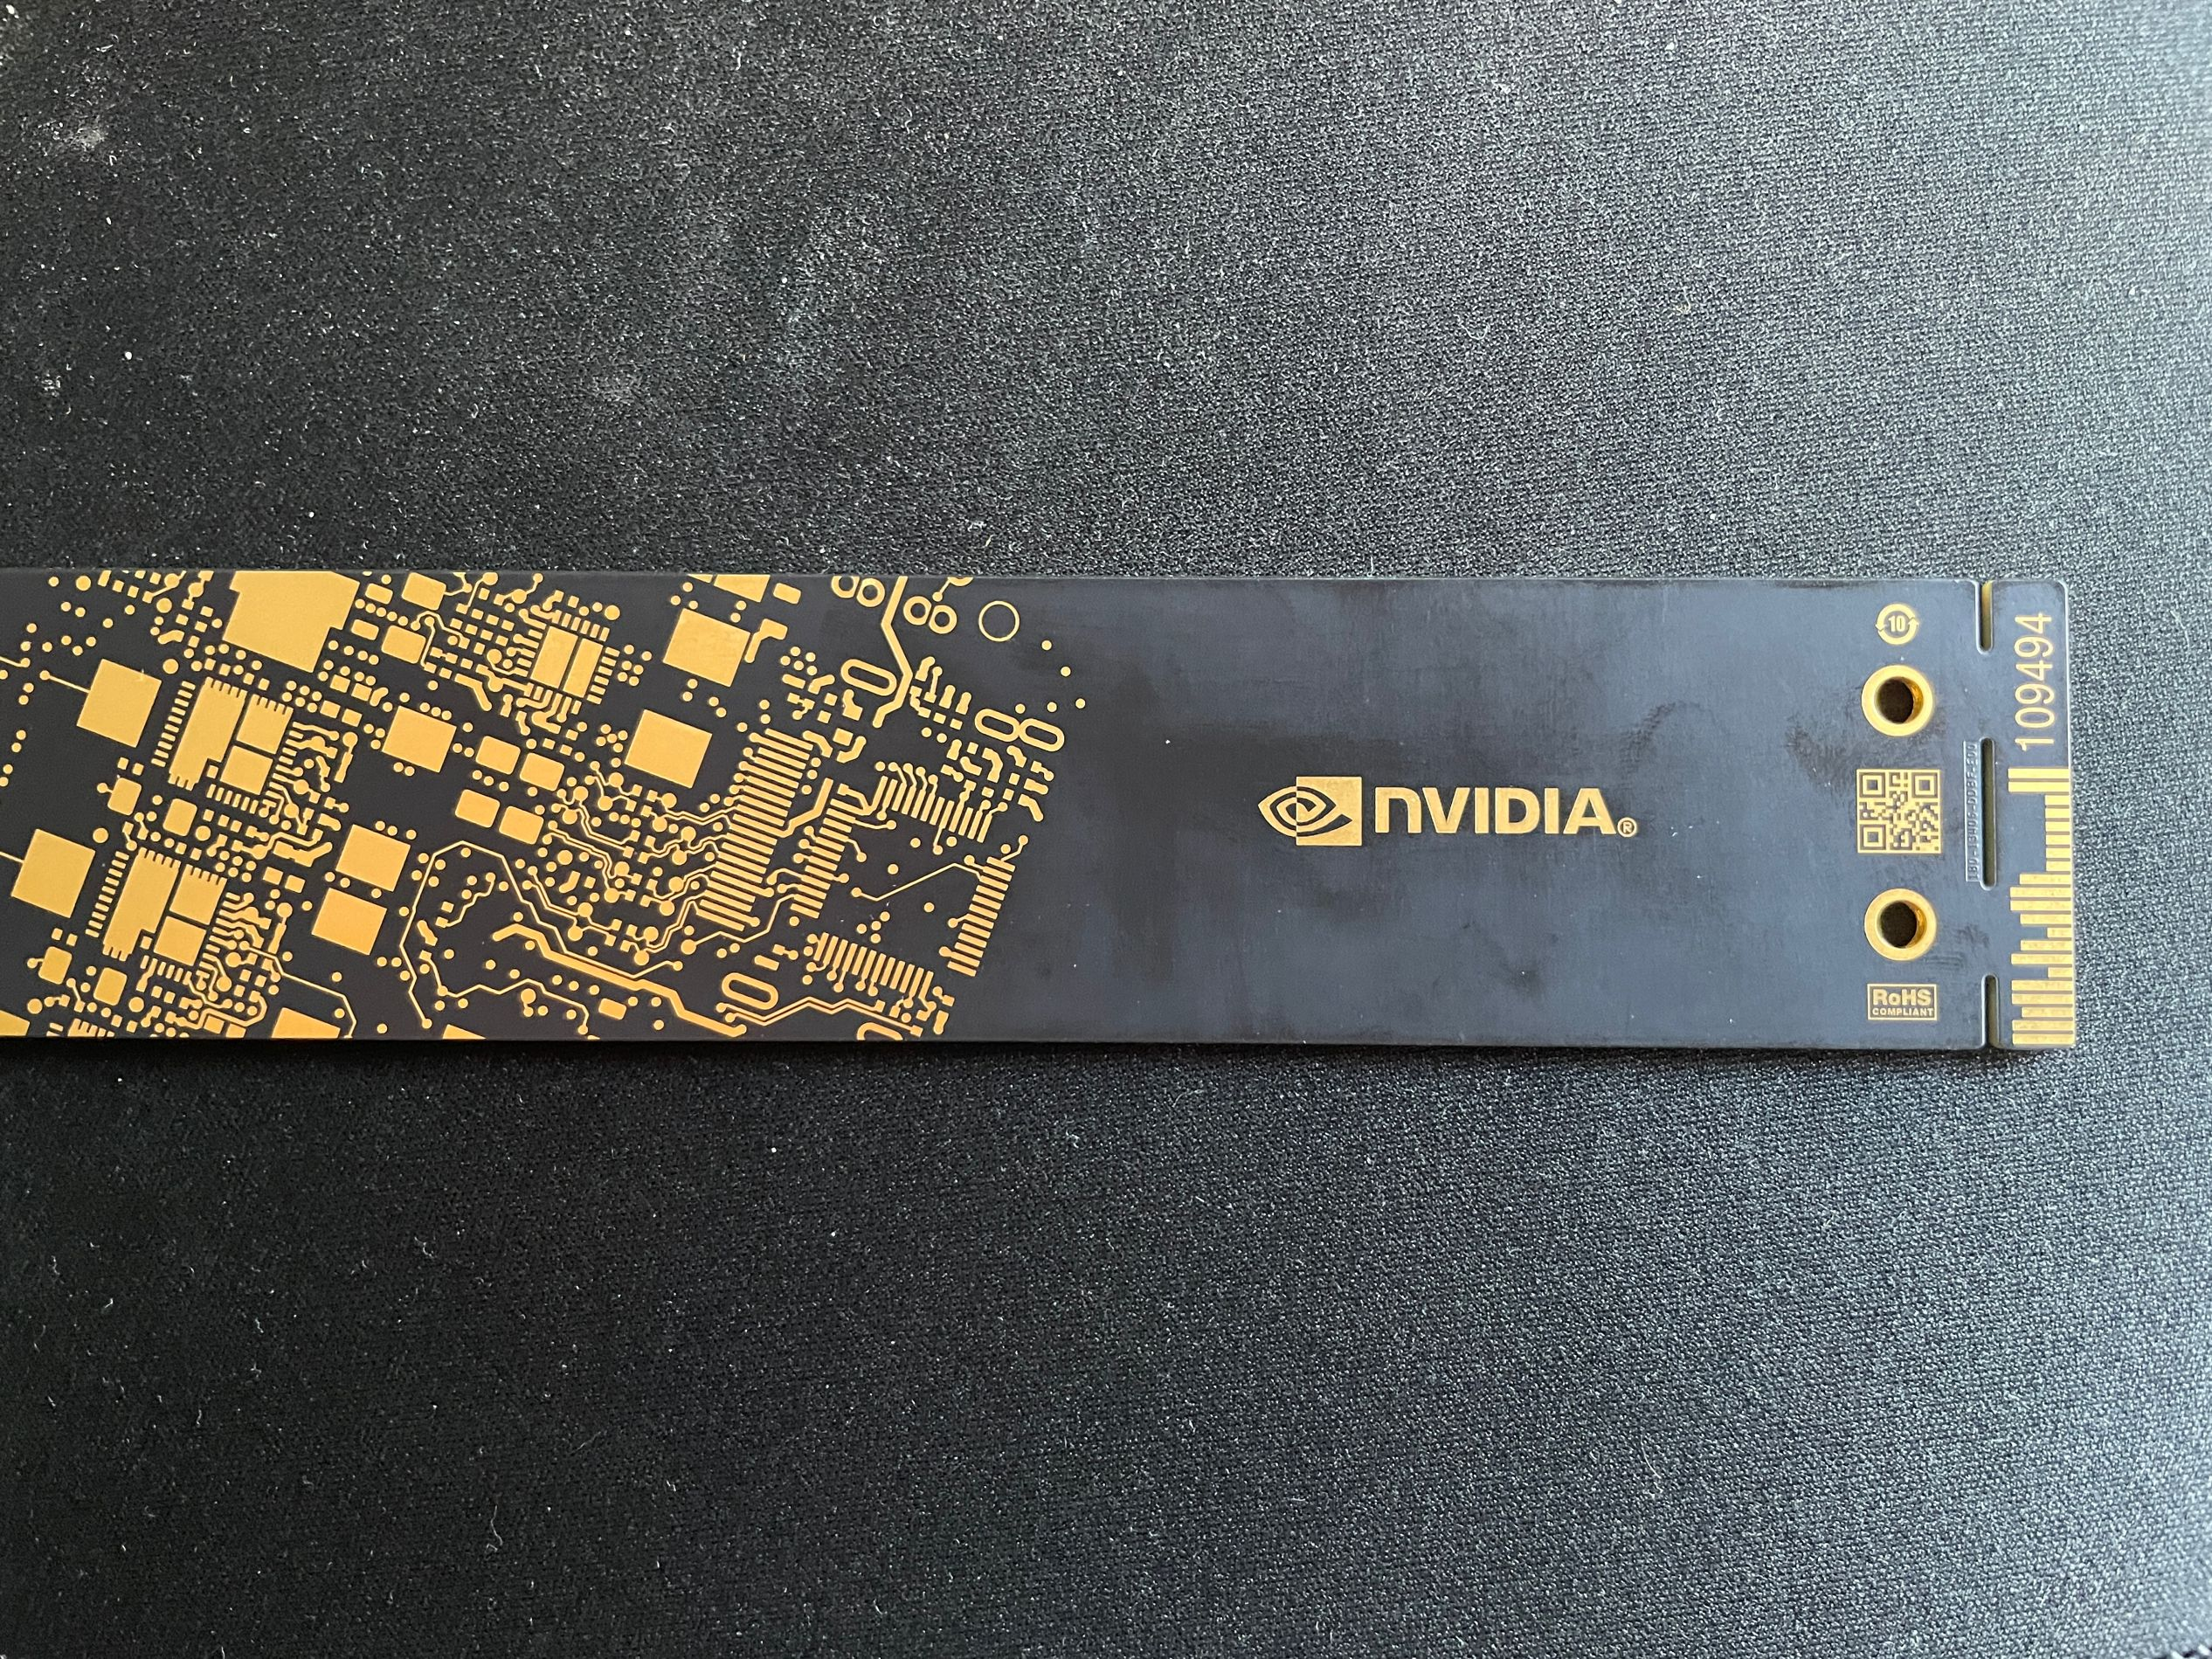
\includegraphics[width=.45\textwidth]{fig/experiment/nvidia-3.jpg}
    }
    \subfigure[提取到的\sift 特征点]{
        \begin{tikzpicture}[spy using outlines={circle, magnification=5, size=40pt, connect spies}]
            \node[anchor=south west, inner sep=0](img) at (0,0){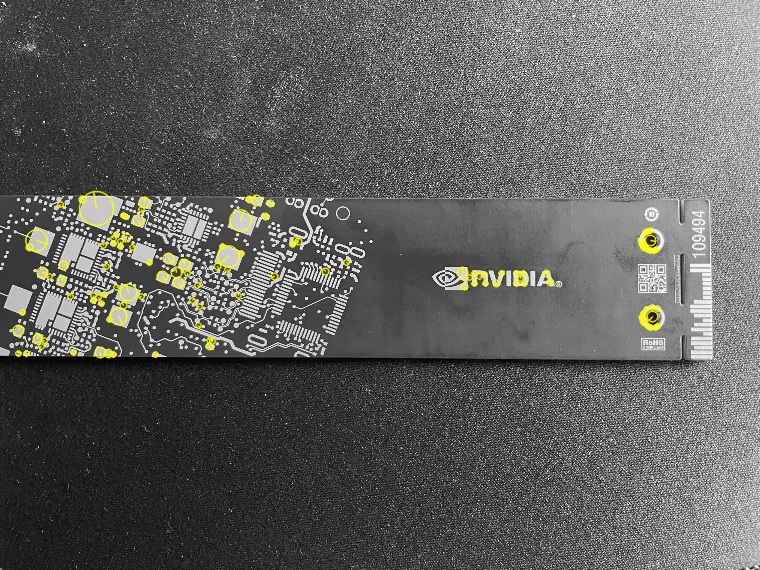
\includegraphics[width=.45\textwidth]{fig/experiment/nvidia-3-keypoints.jpg}};

            \begin{scope}[x={(img.south east)}, y={(img.north west)}]
                % % 绘制坐标辅助网络
                % \drawgrid %

                % 定位缩放点
                % \coordinate (spypoint) at (0.46, 0.66);
                % \coordinate (magnifyglass) at (0.0, 0.0);
            \end{scope}
            \spy [湖蓝, ultra thick] on (1.824,2.48) in node [above] at (4,3);

        \end{tikzpicture}
    }
    \caption{\sift 特征提取结果。观察提取到的关键点,发现它们大多位于角点附近。平均用时$0.1$s。}
\end{figure}

\subsection{特征点匹配}

输入两幅图像,分别对它们进行\sift 特征提取与描述,并在两组描述子之间进行匹配。脚本运行命令示例:
\begin{zshcode}
python image_matching.py \
       --file_dir_1 images/nvidia-3.jpg \ # input image 1
       --file_dir_2 images/nvidia-4.jpg \ # input image 2
       -o 5 \ # number of octaves
       -s 3 \ # number of scales per octave
       --rescale 0.3 \
       --output_dir images/experiment/image_matching.pdf \ # output destination
       --sigma 1.0 \ # use for Gaussian blurring
       -t 0.05 # threshold for detection
\end{zshcode}

结果:
\begin{figure}[H]
    \centering
    \begin{tikzpicture}
        \node[anchor=south west, inner sep=0](img) at (0,0){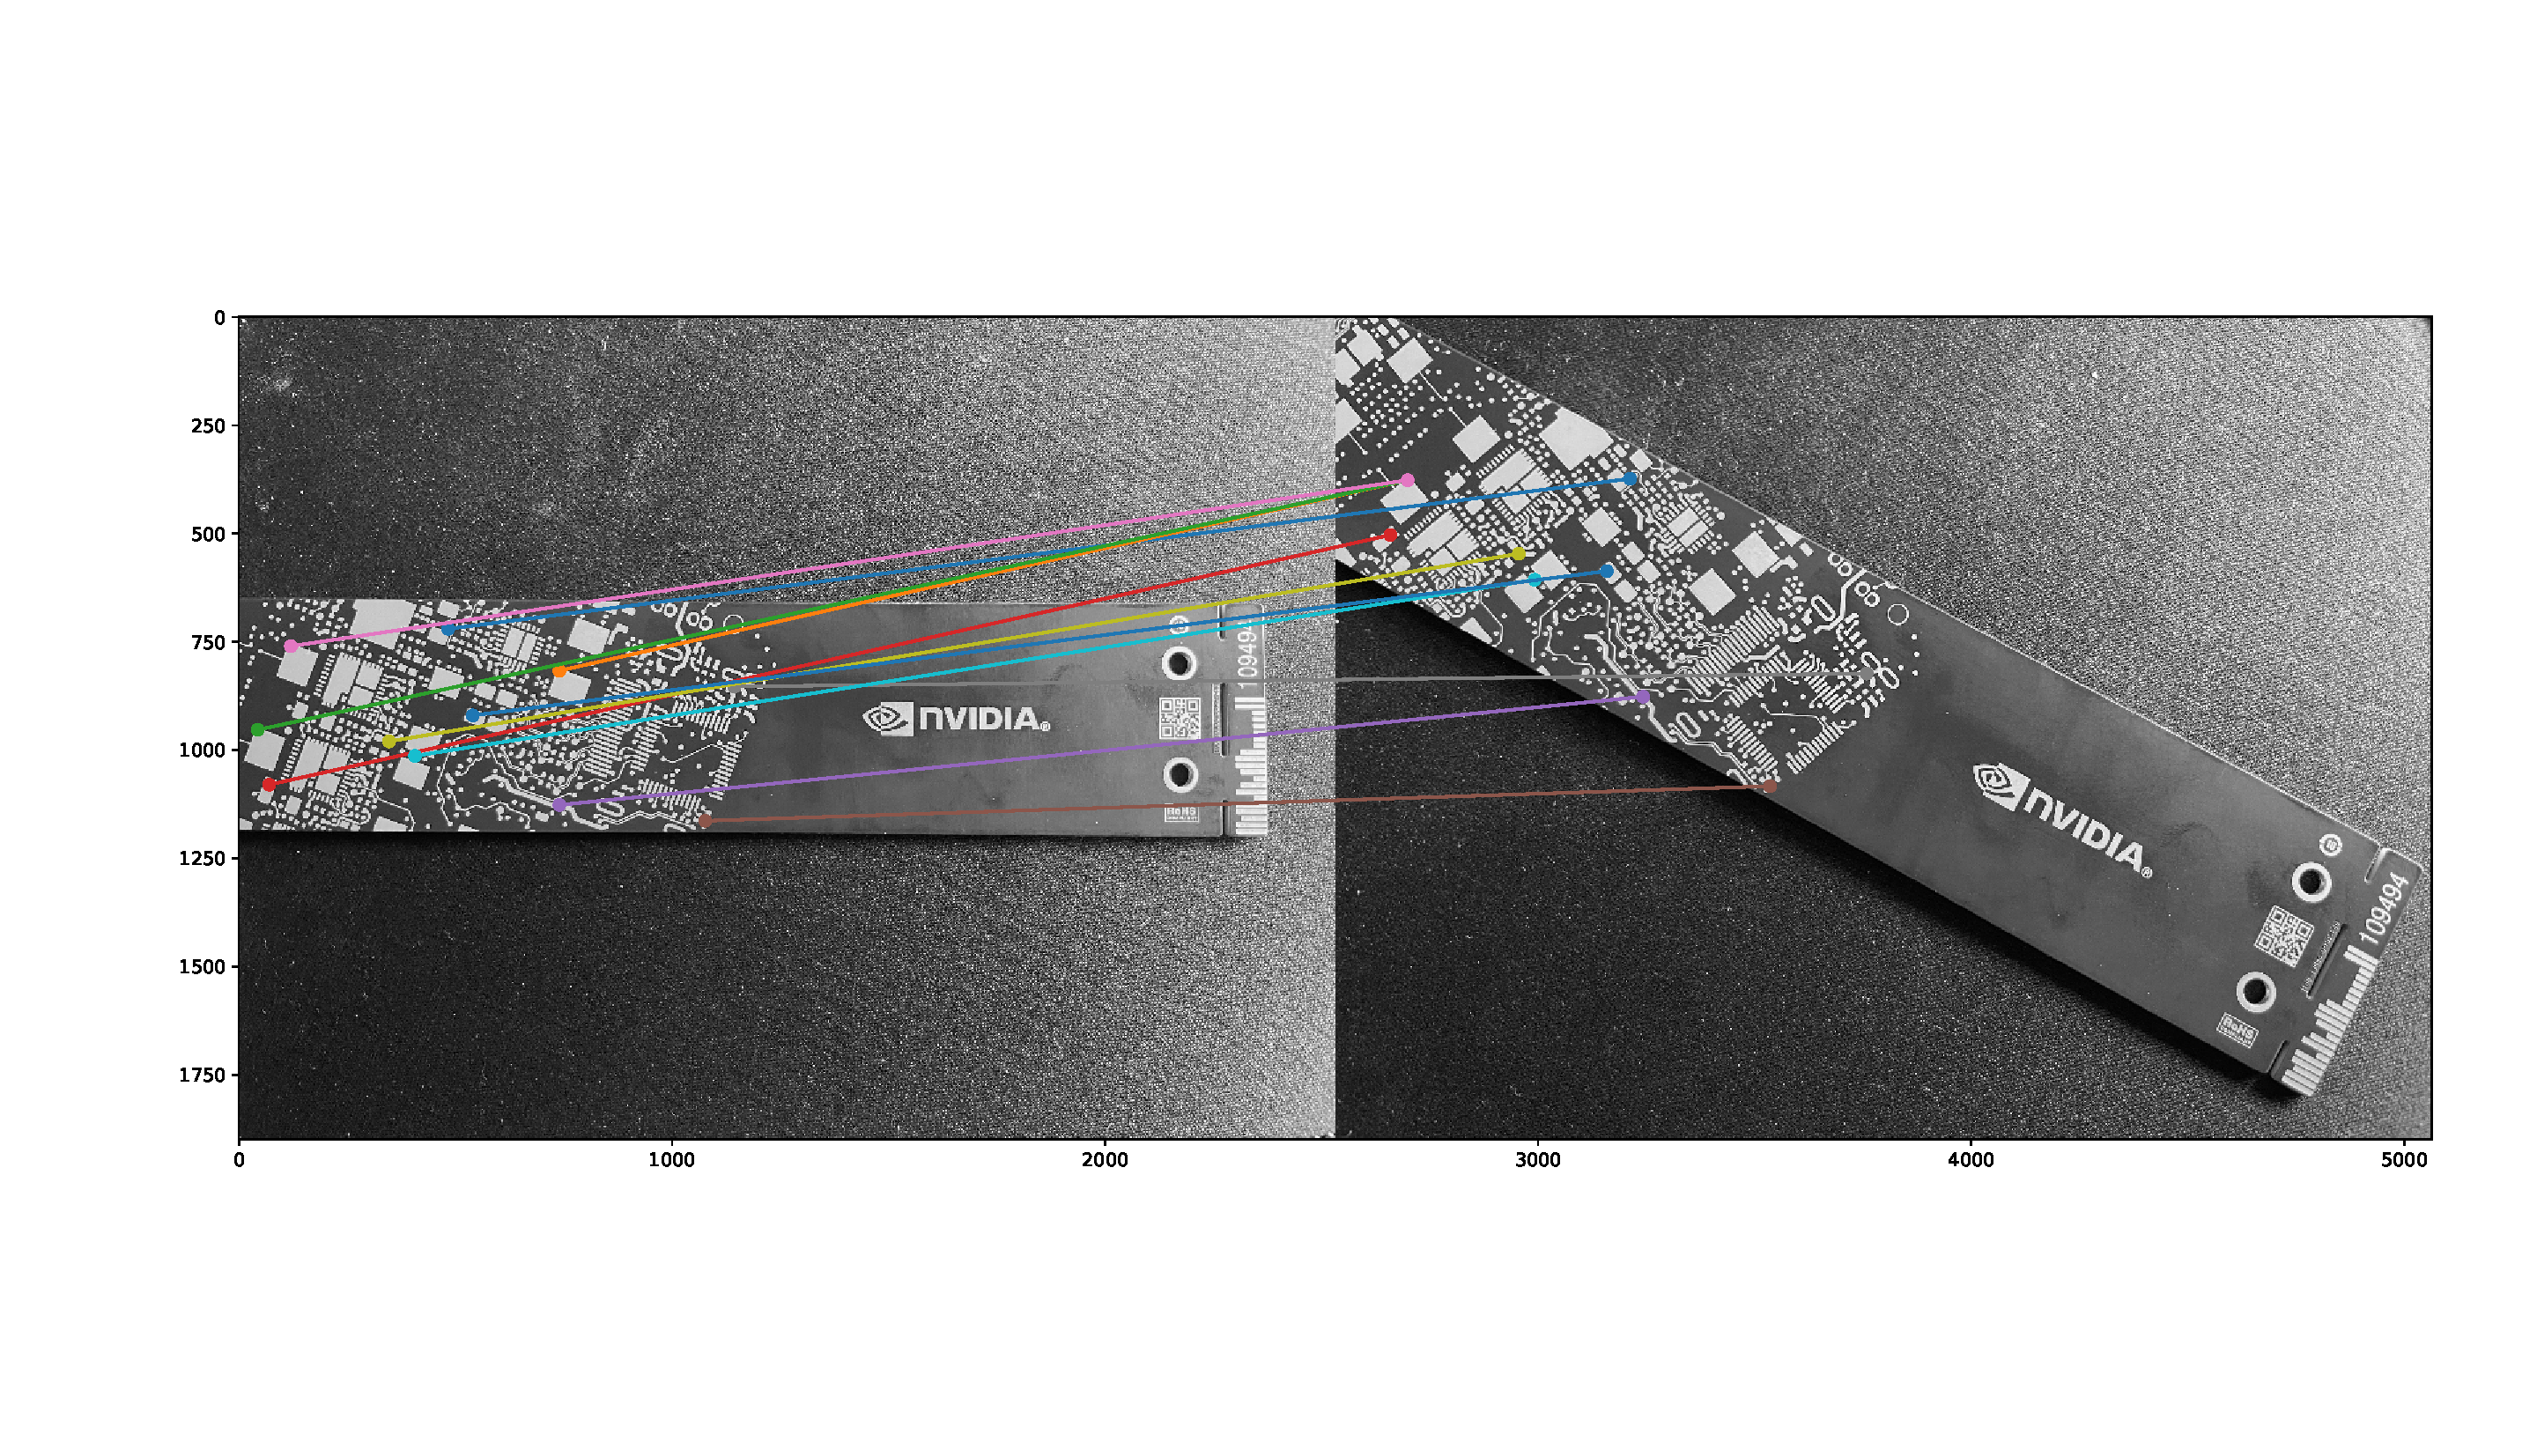
\includegraphics[width=1.1\textwidth]{fig/experiment/image_matching_manual_saving.pdf}};

        \begin{scope}[x={(img.south east)}, y={(img.north west)}]
            % % 绘制坐标辅助网络
            % \drawgrid

            % 定位缩放点
            \coordinate (error1) at (0.039, 0.51);
            \coordinate (error2) at (0.053, 0.603);
            \coordinate (error3) at (0.17, 0.577);
        \end{scope}


        \draw[color=green, ultra thick] (error1) circle (4pt);

        \draw[color=red, ultra thick] (error2) circle (4pt);

        \draw[color=red, ultra thick] (error3) circle (4pt);

    \end{tikzpicture}
    \caption{特征点匹配。右侧的查询图像相比左侧的数据库图像,发生了尺度、旋转上的变化。一共得到9对匹配点,其中错误的匹配有2对(红圈标注),匹配正确率$77.8$\%。平均用时$0.3$s。}
\end{figure}

上述实验中一共获得了9对匹配点,其中错误的匹配有2对(红圈所示),均重复匹配到了另一位置上的特征(绿圈所示)。其原因在于该三处特征的确十分近似,仅仅依靠局部特征将存在定位歧义性。可见\sift 无法对重复的纹理特征进行有效匹配。
